%!TEX root = ../dissertation.tex
\chapter{Thermal conductance in high density graphene}
\label{ch:thermal_conductance_in_high_density_graphene}
When the Fermi level of graphene is doped far from the Dirac point $(\mu\gg k_BT)$, graphene has a well defined Fermi surface and the assumptions in Sommerfeld's derivation of the Lorentz ratio hold. In 2013, Fong et al.~\cite{fong_measurement_2013} verified the Wiedemann-Franz for graphene on SiO$_2$ (Fig.~\ref{fig:Fong_Gth}) using Joule heating and Johnson noise thermometry. The device measured had a mobility of $\mu \gtrsim 5,000~cm^2/Vs$ and a length which emphasized phonon scattering, resulting in the Wiedemann-Franz law (WFL) only being verifiable until $1~K$. Nevertheless, a Lorenz ratio varying between $1-2~\sL_0$ was measured for various charge densities (Fig.~\ref{fig:Fong_Gth}) at low temperature. Above $1~K$ the thermal conductance increased above the WFL due to electron-phonon scattering as described in section~\ref{section:elph}. A few months later, Yigen et al.~\cite{yigen_wiedemannfranz_2014} performed similar Joule heating experiments using resistive thermometry with higher quality suspended graphene ($\mu \gtrsim 35,000~cm^2/Vs$). As shown in Fig.\ref{fig:Yigen}, the shorter device geometry allowed them to measure the WFL to a much higher temperature of ${\sim}150~K$ finding experimental Lorenz ratios of about $0.5~\sL_0$.
\begin{figure}
\centering
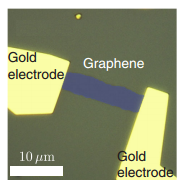
\includegraphics[height=30mm, valign=t]{figures/high_density_graphene/Fong_picture.png}
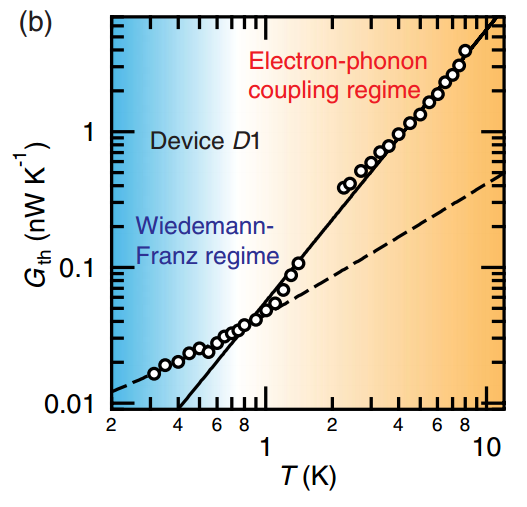
\includegraphics[height=55mm, valign=t]{figures/high_density_graphene/Fong_Gth.png}
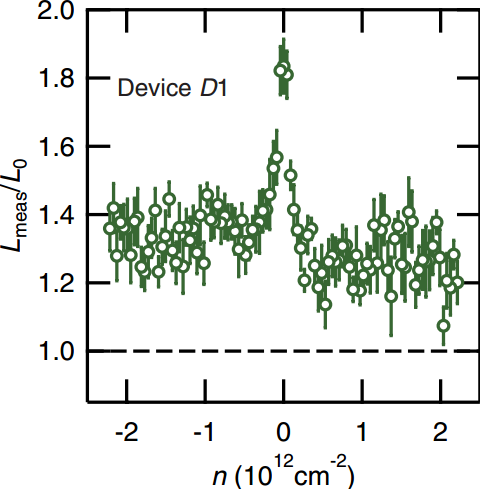
\includegraphics[height=50mm, valign=t]{figures/high_density_graphene/Fong_L.png}
\caption{(\textbf{left}) Device image and (\textbf{center}) electronic thermal conductivity of graphene on SiO$_2$ measured by Fong et al.~\cite{fong_measurement_2013} using Johnson noise thermometry. Dashed line is a fit to the Wiedemann-Franz law. Below $1~K$ the device shows WF behavior while at higher temperature the measured conduction is higher due to phonons coupling. The longer device used in this study resulted in phonons dominating conductance at a lower temperature. (\textbf{right}) The corresponding measured Lorenz ratio vs carrier density. Reprinted under the Creative Commons Attribution 3.0 License from Ref.~\cite{fong_measurement_2013}.}
\label{fig:Fong_Gth}
\end{figure}
\begin{figure}
\centering
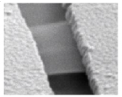
\includegraphics[height=45mm, valign=t]{figures/high_density_graphene/Yigen_picture.png}
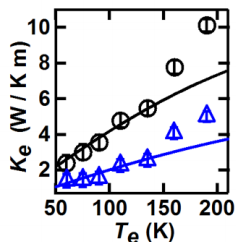
\includegraphics[height=50mm, valign=t]{figures/high_density_graphene/Yigen_Gth.png}
\caption{Electronic thermal conductivity of suspended graphene measured by Yigen et al.~\cite{yigen_wiedemannfranz_2014} using resistive thermometry. Two curves correspond to different carrier densities. Solid lines are fits to the Wiedemann-Franz law. Below ${\sim150}~K$ the device shown WF behavior while at higher temperature the measured conduction is higher due to phonons coupling. Device is $650~nm$ long. Reprinted with permission from \cite{yigen_wiedemannfranz_2014}. Copyright (2014) American Chemical Society.}
\label{fig:Yigen}
\end{figure}

In this chapter we present similar data on higher mobility samples encapsulated with hexagonal boron nitride (hBN).


\section{Device characteristics}
\begin{figure}
\centering
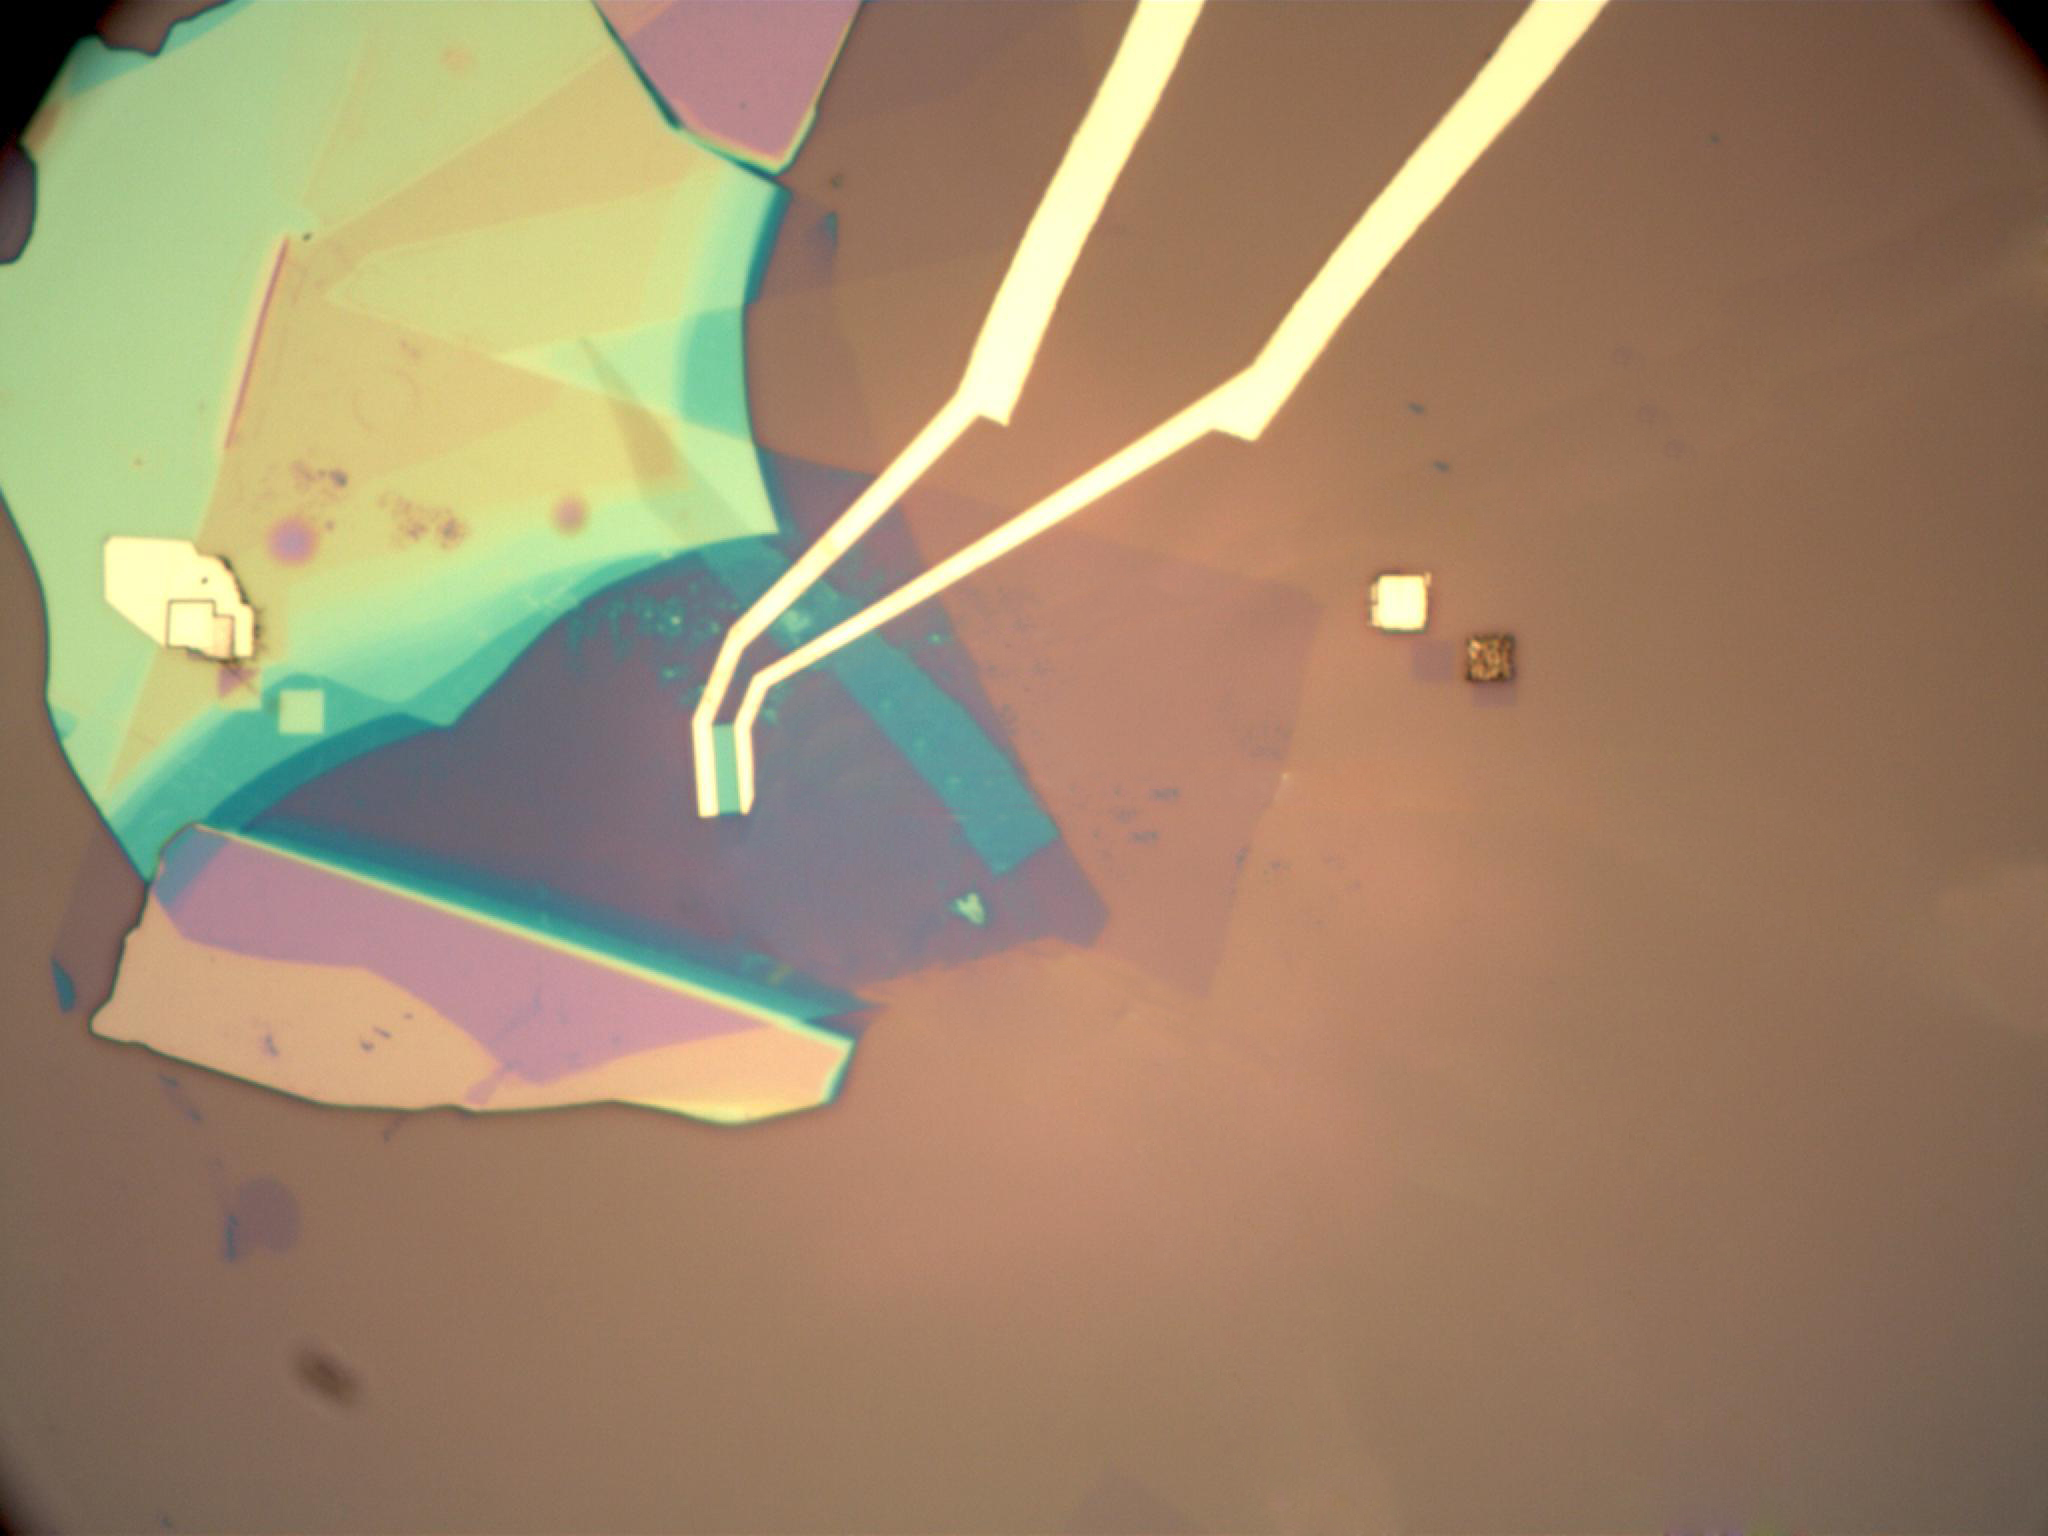
\includegraphics[height=45mm, valign=t]{figures/high_density_graphene/picture_aria.jpg}
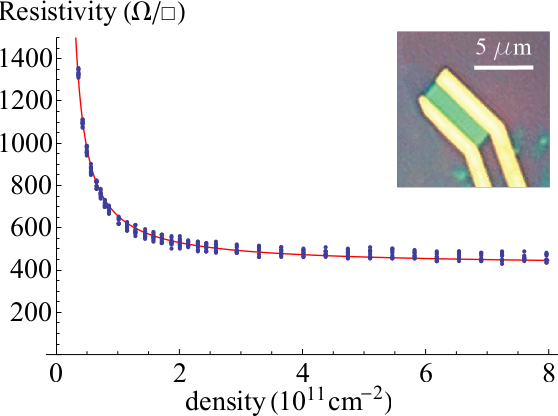
\includegraphics[height=50mm, valign=t]{figures/high_density_graphene/mobility.png}
\caption{(\textbf{left}) Microscope image of the two-terminal graphene device $(2~\mu m\times6~\mu m)$ used in thermal conduction studies presented in this chapter. (\textbf{right}) Estimated resistivity vs carrier density from two-terminal resistance. Solid red line is a fit used to estimate a carrier mobility of $\mu\approx 330,000~cm^2/Vs$.}
\label{fig:Aria}
\end{figure}
Monolayer graphene is mechanically exfoliated, encapsulated in hexagonal boron nitride, and contacted along its 1-dimensional edge~\cite{wang_one-dimensional_2013} to form a $(2~\mu m\times6~\mu m)$ channel (Fig.~\ref{fig:Aria}). A typical two-terminal channel resistance $R$ of this device varies between $150$ and $800~\Omega$ depending on the back gate voltage. The mobility, $\mu$, of the device can be estimated by fitting the two-terminal resistance as a function of charge density $n$, as shown in Fig.~\ref{fig:Aria}, to find $\mu\approx 330,000~cm^2/Vs$ at $3~K$ and $\mu\approx 60,000~cm^2/Vs$ at $300~K$.

As maximal noise power is collected when the device is impedance matched to the measurement chain, an LC tank circuit is placed on chip to transform the graphene to $50~\Omega$ (as disscussed in section~\ref{section:matching} and Refs.~\cite{fong_ultrasensitive_2012} and  \cite{schoelkopf_radio-frequency_1998}) within the measurement bandwidth. The matching network defines a bandwidth of ${25~MHz}$ centered at ${133~MHz}$, as shown in Fig.~\ref{fig:Aria_matching}. The total noise power emitted into this bandwidth is amplified and measured via the circuit and procedure outlined in chapter~\ref{ch:thermal_conductance_via_electrical_noise} resulting in a measured output voltage (proportional to the total noise power) similar to that shown in Fig.~\ref{fig:Aria_noise}

\begin{figure}
\centering
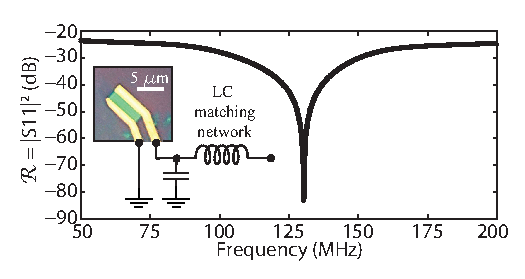
\includegraphics[width=80mm]{figures/high_density_graphene/matching.eps}
\caption{RF reflectance off the two-terminal graphene device presented in this chapter. The sample impedance is transformed using a single stage LC network (inset) resulting in a measurement bandwidth of $25~MHz$ centered at $133~MHz$. See section~\ref{section:matching} for details on impedance matching.}
\label{fig:Aria_matching}
\end{figure}

\begin{figure}
\centering
\includegraphics[width=80mm]{figures/high_density_graphene/noise.eps}
\caption{Measured DC voltage proportional to the total noise emitted from a graphene device as a function of bath temperature and back gate voltage using the circuit outline in chapter~\ref{ch:johnson_noise_thermometry}.}
\label{fig:Aria_noise}
\end{figure}

\section{Thermal conductance}
For the results shown here, the graphene device is measured away from the charge neutrality point with hole density $n\approx5.7\times 10^{10}cm^{-2}$, where $R$ varies between $280$ and $480~\Omega$ from $3$ to $300~K$. The Johnson noise thermometer is calibrated to a given sample following the procedure outlined in chapter~\ref{ch:johnson_noise_thermometry} and the thermal conductance, $G_{th}$, is extracted as discussed in chapter~\ref{ch:thermal_conductance_via_electrical_noise}.

The measured thermal conductance of our device falls into two temperature regimes as shown in Fig.~\ref{fig:Aria_Gth}. For $T<100~K$, $G_{th}$ linearly depends on temperature and is well described by the Wiedemann-Franz law. The dashed line in the left panel of Fig.~\ref{fig:Aria_Gth} shows the theoretical Wiedemann-Franz conductance ($G_{WF}$) with an offset of $0.015~\mu\Watt/K$. The fitted~\cite{fong_measurement_2013, yigen_wiedemannfranz_2014} Lorenz number is $2.38\times10^{-8} \Watt\Omega K^{-2}$, $3\%$ below the theoretical value. As the charge density is swept, the Lorenz ratio varies similar to that seen in ref~\cite{fong_measurement_2013}, always remaining close to$\sL_0$.
\begin{figure}
\centering
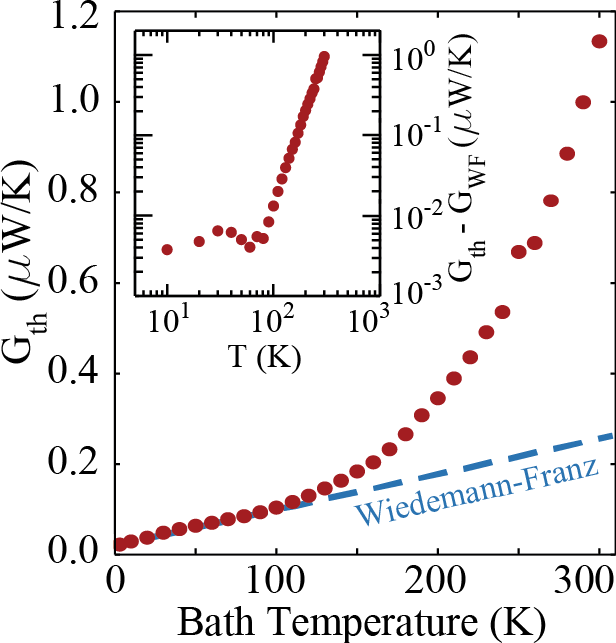
\includegraphics[height=50mm, valign=t]{figures/high_density_graphene/Gth_lin.png}
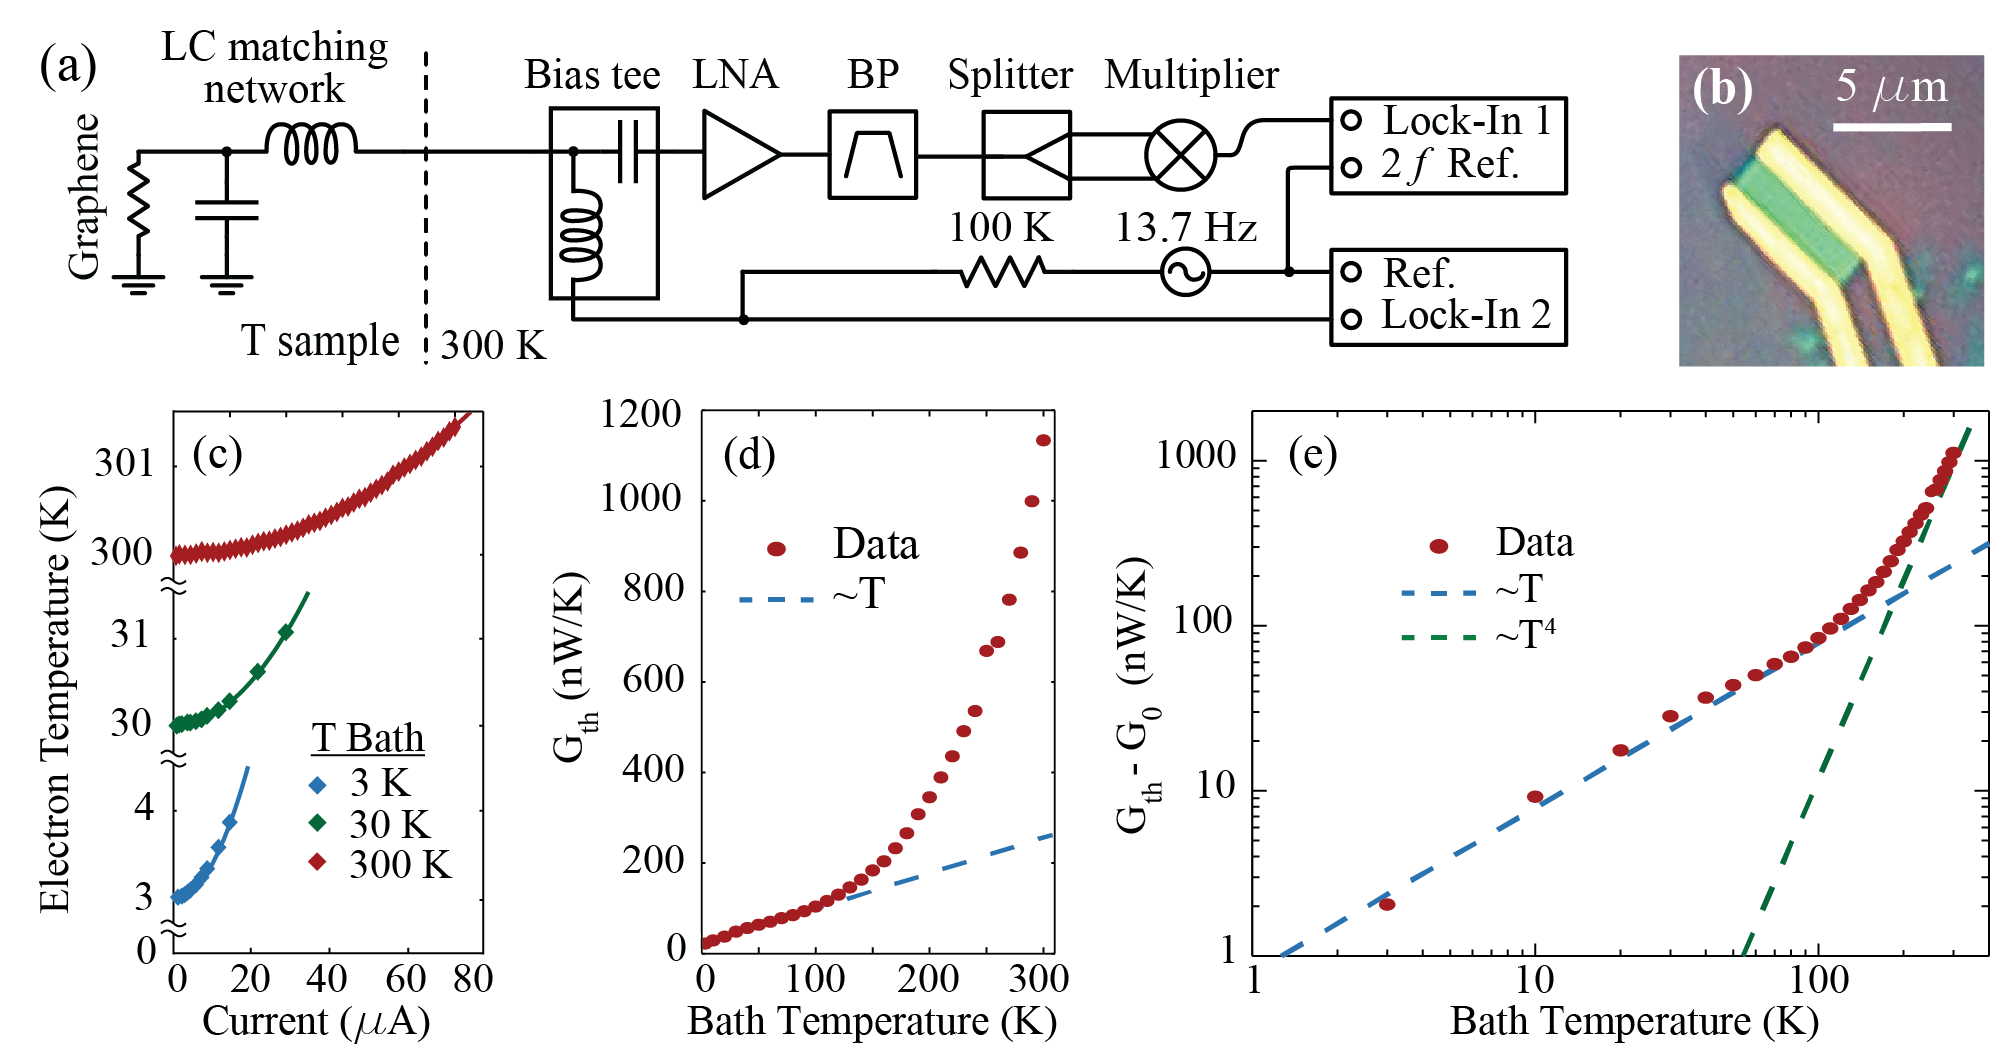
\includegraphics[height=50mm, valign=t]{figures/high_density_graphene/Gth_log.png}
\caption{(\textbf{left}) Graphene thermal conductance from $3~K$ to $300~K$. Blue dashed line shows the theoretical Wiedemann-Franz conductance for our device geometry offset by a fitted constant. (\textbf{Inset}) shows the total conductance with $G_{WF}$ subtracted. Above $T\sim 80~K$, the conductance departs with a power law of $3.88 \pm 0.02$. (\textbf{right}) Same data with the fitted offset removed, shown on a log-log scale.}
\label{fig:Aria_Gth}
\end{figure}

At higher temperature, the measured $G_{th}$ is larger than Wiedemann-Franz conductance indicating a different energy transfer mechanism dominates above $100~K$. Fig.~\ref{fig:Aria_Gth}(right) shows the same data on a log-log plot making clear the two different power laws in the different regimes. To extract the electron-phonon coupling constants, as outlined in section~\ref{section:elph}, the thermal conductance from electron diffusion must be accounted for. Fig.~\ref{fig:Aria_Gth} inset plots $G_{th}$ with $G_{WF}$ subtracted. $G_{th}$ departs from $G_{WF}$ with a fitted power law of $3.88\pm0.02$ and an amplitude of  $0.23\pm 0.03~{f\Watt}/K^{4.88}$. We note that the high power law $\delta\approx4$ in our measured data is in sharp contrast to the sublinear temperature dependence of graphene's lattice conductivity for $T>150~K$~\cite{seol_two-dimensional_2010}, suggesting that it is unlikely the energy transfer bottleneck and hence the lattice is well thermalized to the bath. 

We compare the high temperature thermal conductance of our sample with the expected contributions from acoustic phonons~\cite{bistritzer_electronic_2009, viljas_electron-phonon_2010} and the supercollision cooling mechanism~\cite{song_disorder-assisted_2012, chen_electron-phonon_2012, betz_supercollision_2013, graham_photocurrent_2013} given the measured mobility in Fig.~\ref{fig:Aria_Eph}; We estimate these contributions to be an order of magnitude too small to explain the observed $G_{th}$. From our experiment, we estimate that the thermal conductance per unit area at $300~K$ to be $9.5\times10^{4}~\Watt/Km^{2}$. We find this to be comparable to theoretical calculations which suggest that optical phonons, both in the graphene lattice and the boron nitride substrate, may provide an energy relaxation channel substantially larger than acoustic phonons in this high temperature limit~\cite{sohier_phonon-limited_2014, tielrooij_out--plane_2017, viljas_electron-phonon_2010, bistritzer_electronic_2009, schiefele_temperature_2012}.
\begin{figure}
\centering
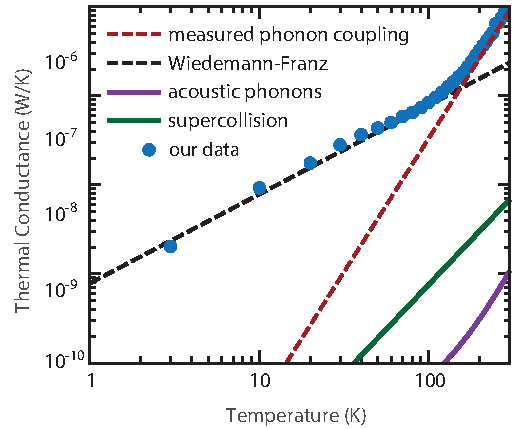
\includegraphics[width = 80mm]{figures/high_density_graphene/EPh.pdf}
\caption{Thermal conductance of a graphene device compared to estimated contributions from acoustic phonons~\cite{bistritzer_electronic_2009, viljas_electron-phonon_2010} and the supercollision cooling mechanism~\cite{song_disorder-assisted_2012, chen_electron-phonon_2012, betz_supercollision_2013, graham_photocurrent_2013}.}
\label{fig:Aria_Eph}
\end{figure}